\chapter {Introduction to Partial Derivative}

Let $f(x, y)$ be a function of two variables, the partial derivative of $f$
with respect to $x$ is defined as \[\frac{\partial f}{\partial x} = \lim_{h \to 0} \frac{f(x + h, y) - f(x, y)}{h}\] if the limit exists. Similarly, the partial derivative of $f$ with respect to
$y$ is defined as \[\frac{\partial f}{\partial y} = \lim_{h \to 0} \frac{f(x, y + h) - f(x, y)}{h}\] if the limit exists. It is the rate of change of $f$ with respect to $x$ and
$y$ respectively with one variable held constant. Intuitively, it is the slope
of the tangent line of $f$ in the $x$ and $y$ direction respectively. Same can
be done for functions of more than two variables.

Imagine a surface $z = f(x, y)$ in the $xyz$-space and a point $P(x_0, y_0,
    z_0)$ on the surface. Now cut the surface with a plane perpendicular to the
$xy$-plane and parallel to the $x$-axis at $x = x_0$. The curve of intersection
of the surface and the plane is called the trace of the surface on the plane.
The slope of the tangent line of the trace at $P$ is $\frac{\partial f}{\partial x}(x_0, y_0)$. Similarly, same can be done for the $y$-axis.

\begin{center}
    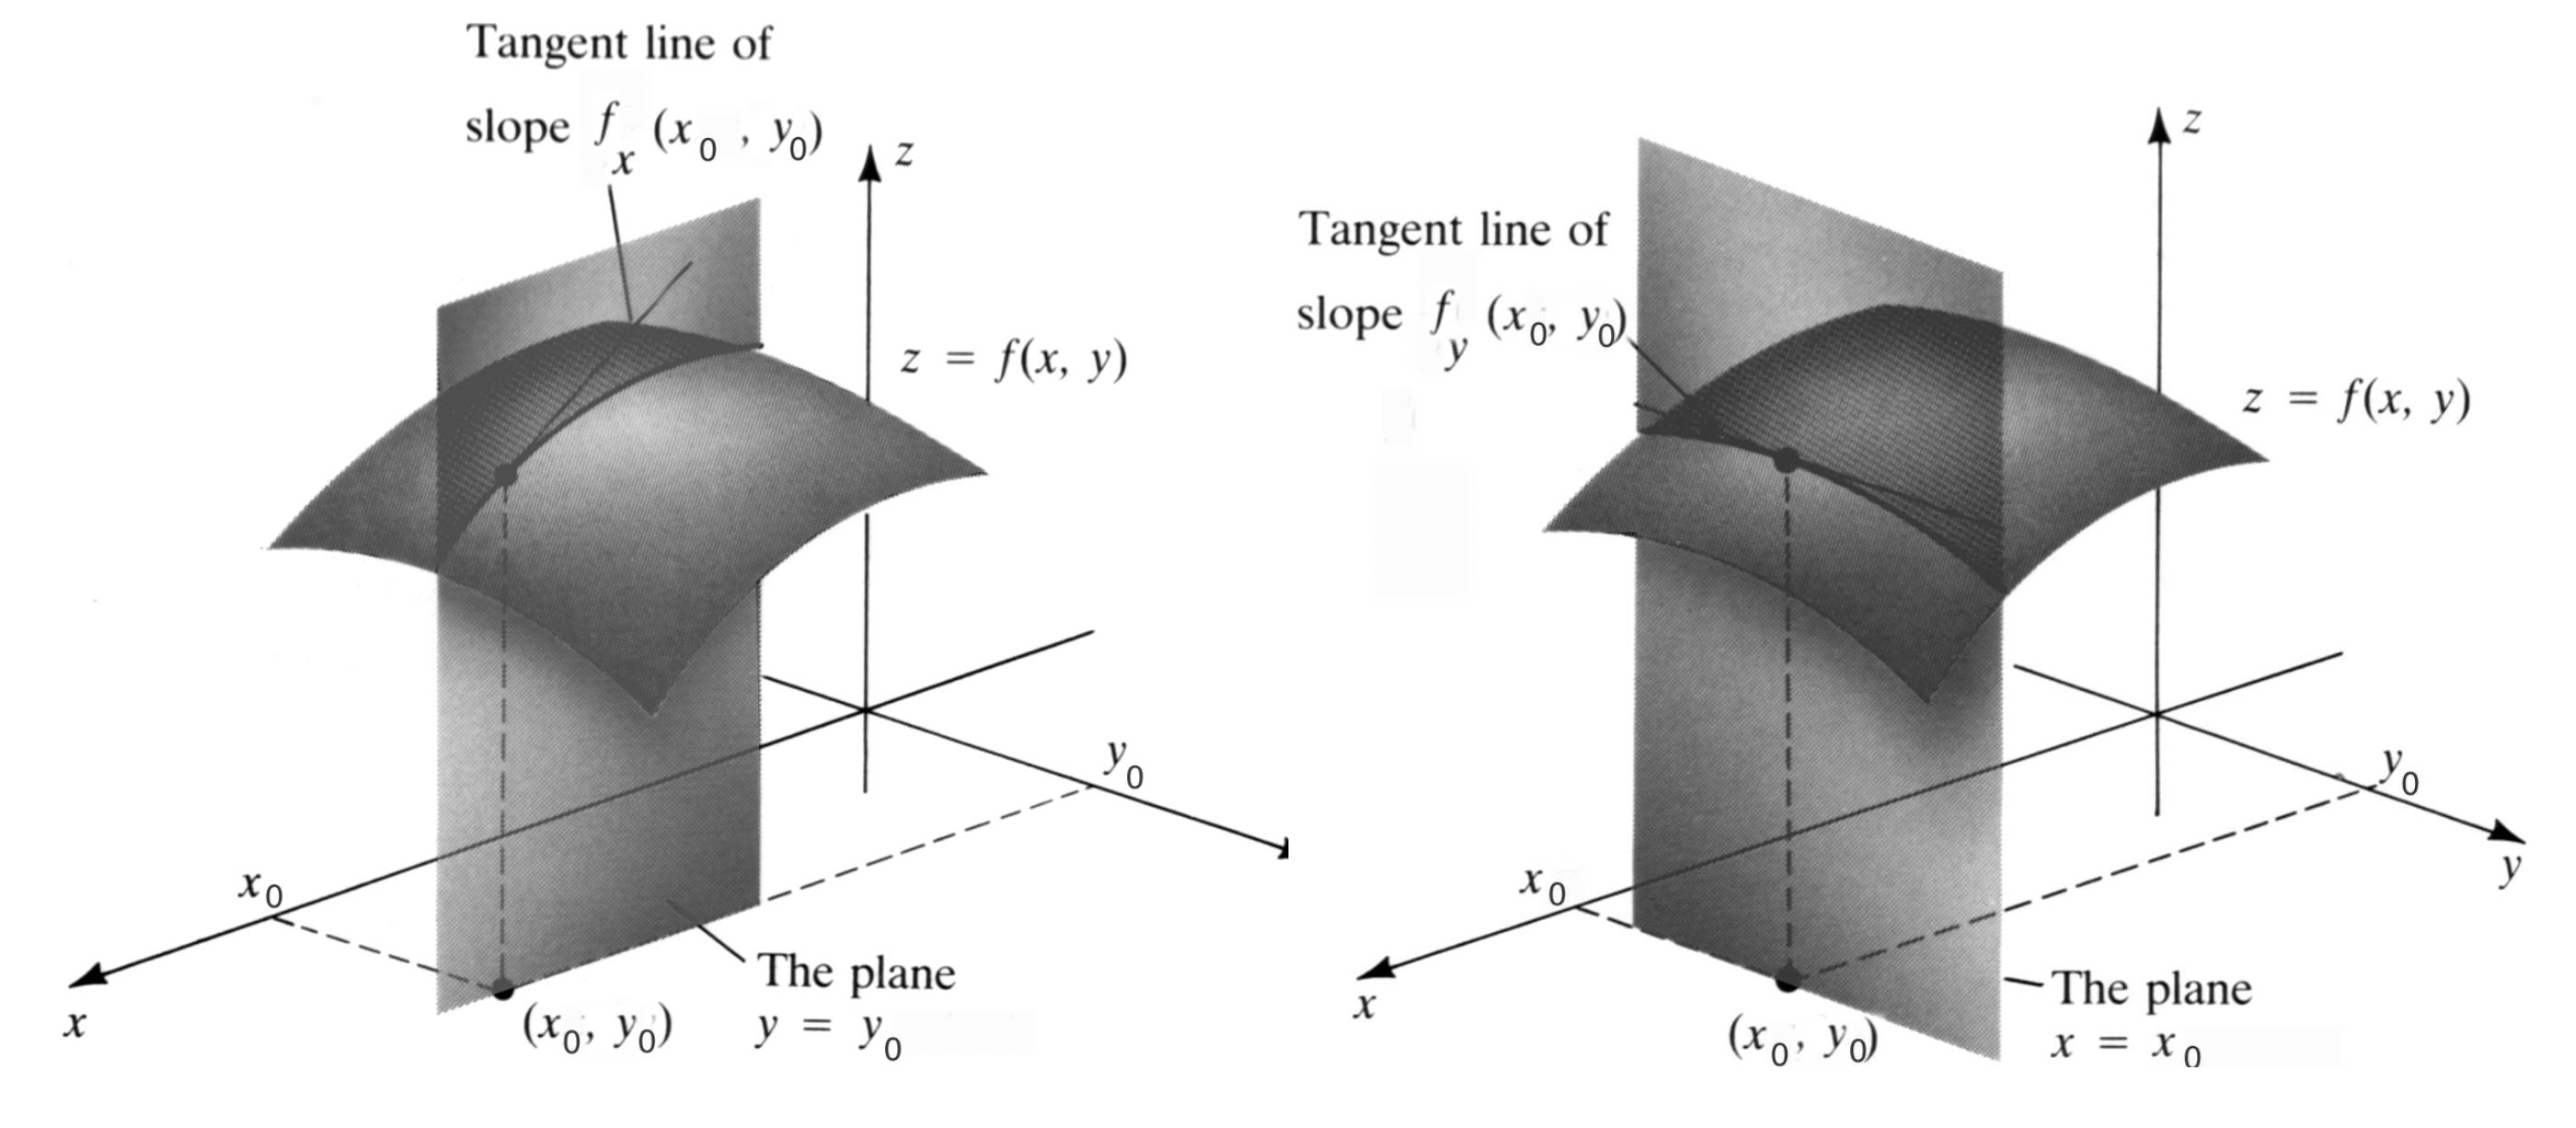
\includegraphics[scale=0.15]{assets/Partial Derivative.png}
\end{center}

\newpage
\section*{Selected Exercises}
\textit{Source: Larson Calculus 11th Ed. Exercise 13.3}

\begin{enumerate}[label={}, leftmargin=*]
    \item \textbf{Finding Partial Derivatives} In Exercises 11-40, find both first partial derivatives.
\end{enumerate}
\begin{enumerate}
    \item $f(x, y)=2 x-5 y+3$
          \sol{}
          \begin{align*}
              \frac{\partial f}{\partial x} & = 2 \\ \frac{\partial f}{\partial y} &= -5
          \end{align*}

    \item $f(x, y)=x^2-2 y^2+4$
          \sol{}
          \begin{align*}
              \frac{\partial f}{\partial x} & = 2x \\ \frac{\partial f}{\partial y} &= -4y
          \end{align*}

    \item $z=6 x-x^2 y+8 y^2$
          \sol{}
          \begin{align*}
              \frac{\partial f}{\partial x} & = 6-2xy \\ \frac{\partial f}{\partial y} &= -x^2+16y
          \end{align*}

    \item $f(x, y)=4 x^3 y^{-2}$
          \sol{}
          \begin{align*}
              \frac{\partial f}{\partial x} & = 12x^2y^{-2} \\ \frac{\partial f}{\partial y} &= -8x^3y^{-3}
          \end{align*}

    \item $z=x \sqrt{y}$
          \sol{}
          \begin{align*}
              \frac{\partial f}{\partial x} & = \sqrt{y} \\ \frac{\partial f}{\partial y} &= \frac{x}{2\sqrt{y}}
          \end{align*}
          \newpage
    \item $z=2 y^2 \sqrt{x}$
          \sol{}
          \begin{align*}
              \frac{\partial f}{\partial x} & = \frac{y^2}{\sqrt{x}} \\ \frac{\partial f}{\partial y} &= 4y\sqrt{x}
          \end{align*}

    \item $z=e^{x y}$
          \sol{}
          \begin{align*}
              \frac{\partial f}{\partial x} & = y e^{xy} \\ \frac{\partial f}{\partial y} &= x e^{xy}
          \end{align*}

    \item $z=e^{x / y}$
          \sol{}
          \begin{align*}
              \frac{\partial f}{\partial x} & = \frac{1}{y} e^{x/y} \\ \frac{\partial f}{\partial y} &= -\frac{x}{y^2} e^{x/y}
          \end{align*}

    \item $z=x^2 e^{2 y}$
          \sol{}
          \begin{align*}
              \frac{\partial f}{\partial x} & = 2x e^{2y} \\ \frac{\partial f}{\partial y} &= 2x^2 e^{2y}
          \end{align*}

    \item $z=7 y e^{y / x}$
          \sol{}
          \begin{align*}
              \frac{\partial f}{\partial x} & = -\frac{7y}{x^2} e^{y/x} \\ \frac{\partial f}{\partial y} &= 7e^{y/x} + \frac{7y}{x} e^{y/x}
          \end{align*}

    \item $z=\ln \dfrac{x}{y}$
          \sol{}
          \begin{align*}
              \frac{\partial f}{\partial x} & = \frac{1}{y}\cdot\frac{y}{x} = \frac{1}{x} \\ \frac{\partial f}{\partial y} &= -\frac{x}{y^2} \cdot \frac{y}{x} = -\frac{1}{y}
          \end{align*}

          \newpage
    \item $z=\ln \sqrt{x y}$
          \sol{}
          \begin{align*}
              \frac{\partial f}{\partial x} & = \frac{1}{\sqrt{xy}} \cdot \frac{1}{2\sqrt{xy}} \cdot y =
              \frac{1}{2x}                                                                               \\ \frac{\partial f}{\partial y} & = \frac{1}{\sqrt{xy}} \cdot \frac{1}{2\sqrt{xy}} \cdot x =
                 \frac{1}{2y}
          \end{align*}

    \item $z=\ln \left(x^2+y^2\right)$
          \sol{}
          \begin{align*}
              \frac{\partial f}{\partial x} & = \frac{2x}{x^2+y^2} \\ \frac{\partial f}{\partial y} &= \frac{2y}{x^2+y^2}
          \end{align*}

    \item $z=\ln \dfrac{x+y}{x-y}$
          \sol{}
          \begin{align*}
              \frac{\partial f}{\partial x} & = \dfrac{\partial}{\partial x}[\ln (x + y)] - \dfrac{\partial}{\partial x}[\ln (x - y)] \\  & = \frac{1}{x+y} - \frac{1}{x-y} = \frac{2y}{x^2-y^2}
              \\ \frac{\partial f}{\partial y} & = \dfrac{\partial}{\partial y}[\ln (x + y)] - \dfrac{\partial}{\partial y}[\ln (x - y)] \\ & = \frac{1}{x+y} + \frac{1}{x-y} = \frac{2x}{x^2-y^2}
          \end{align*}
    \item $z=\dfrac{x^2}{2 y}+\dfrac{3 y^2}{x}$
          \sol{}
          \begin{align*}
              \frac{\partial f}{\partial x} & = \frac{x}{y} - \frac{3y^2}{x^2} \\ \frac{\partial f}{\partial y} &= -\frac{x^2}{2y^2} + \frac{6y}{x}
          \end{align*}
    \item $z=\dfrac{x y}{x^2+y^2}$
          \sol{}
          \begin{align*}
              \frac{\partial f}{\partial x} & = \frac{y(x^2+y^2) - xy(2x)}{(x^2+y^2)^2} = \frac{y^3 -
              x^2y}{(x^2+y^2)^2}                                                                      \\ \frac{\partial f}{\partial y} & = \frac{x(x^2+y^2) - xy(2y)}{(x^2+y^2)^2} = \frac{x^3 -
                     xy^2}{(x^2+y^2)^2}
          \end{align*}

          \newpage
    \item $h(x, y)=e^{-\left(x^2+y^2\right)}$
          \sol{}
          \begin{align*}
              \frac{\partial h}{\partial x} & = -2xe^{-\left(x^2+y^2\right)} \\ \frac{\partial h}{\partial y} &= -2ye^{-\left(x^2+y^2\right)}
          \end{align*}

    \item $g(x, y)=\ln \sqrt{x^2+y^2}$
          \sol{}
          \begin{align*}
              \frac{\partial g}{\partial x} & = \frac{1}{\sqrt{x^2+y^2}} \cdot \frac{1}{2\sqrt{x^2+y^2}} \cdot 2x =
              \frac{x}{x^2+y^2}                                                                                     \\ \frac{\partial g}{\partial y} & = \frac{1}{\sqrt{x^2+y^2}} \cdot \frac{1}{2\sqrt{x^2+y^2}} \cdot 2y =
                 \frac{y}{x^2+y^2}
          \end{align*}

    \item $f(x, y)=\sqrt{x^2+y^2}$
          \sol{}
          \begin{align*}
              \frac{\partial f}{\partial x} & = \frac{x}{\sqrt{x^2+y^2}} \\ \frac{\partial f}{\partial y} &= \frac{y}{\sqrt{x^2+y^2}}
          \end{align*}

    \item $f(x, y)=\sqrt{2 x+y^3}$
          \sol{}
          \begin{align*}
              \frac{\partial f}{\partial x} & = \frac{1}{2\sqrt{2x+y^3}} \cdot 2 = \frac{1}{\sqrt{2x+y^3}} \\
              \frac{\partial f}{\partial y} & = \frac{3y^2}{2\sqrt{2x+y^3}}
          \end{align*}

    \item $z=\cos x y$
          \sol{}
          \begin{align*}
              \frac{\partial f}{\partial x} & = -y\sin xy \\ \frac{\partial f}{\partial y} &= -x\sin xy
          \end{align*}

    \item $z=\sin (x+2 y)$
          \sol{}
          \begin{align*}
              \frac{\partial f}{\partial x} & = \cos (x+2y) \\ \frac{\partial f}{\partial y} &= 2\cos (x+2y)
          \end{align*}

    \item $z=\tan (2 x-y)$
          \sol{}
          \begin{align*}
              \frac{\partial f}{\partial x} & = 2\sec^2 (2x-y) \\ \frac{\partial f}{\partial y} &= -\sec^2 (2x-y)
          \end{align*}

    \item $z=\sin 5 x \cos 5 y$
          \sol{}
          \begin{align*}
              \frac{\partial f}{\partial x} & = 5\cos 5x \cos 5y \\ \frac{\partial f}{\partial y} &= -5\sin 5x \sin 5y
          \end{align*}

    \item $z=e^y \sin 8 x y$
          \sol{}
          \begin{align*}
              \frac{\partial f}{\partial x} & = 8ye^y \cos 8xy \\ \frac{\partial f}{\partial y} &= e^y \sin 8xy + 8xe^y \cos 8xy
          \end{align*}

    \item $z=\cos \left(x^2+y^2\right)$
          \sol{}
          \begin{align*}
              \frac{\partial f}{\partial x} & = -2x\sin (x^2+y^2) \\ \frac{\partial f}{\partial y} &= -2y\sin (x^2+y^2)
          \end{align*}

    \item $z=\sinh (2 x+3 y)$
          \sol{}
          \begin{align*}
              \frac{\partial f}{\partial x} & = 2\cosh (2x+3y) \\ \frac{\partial f}{\partial y} &= 3\cosh (2x+3y)
          \end{align*}

    \item $z=\cosh x y^2$
          \sol{}
          \begin{align*}
              \frac{\partial f}{\partial x} & = y^2\sinh xy^2 \\ \frac{\partial f}{\partial y} &= 2xy\cosh xy^2
          \end{align*}

          \newpage
    \item $f(x, y)=\displaystyle\int_x^y\left(t^2-1\right) d t$
          \sol{}
          \begin{align*}
              f(x, y)                       & =\int_x^y\left(t^2-1\right) d t         \\
                                            & = \left[\frac{t^3}{3} - t\right]_x^y    \\
                                            & = \frac{y^3}{3} - y - \frac{x^3}{3} + x \\
              \frac{\partial f}{\partial x} & = -x^2 + 1                              \\ \frac{\partial f}{\partial y} &= y^2 - 1
          \end{align*}

    \item $f(x, y)=\displaystyle\int_x^y(2 t+1) d t+\int_y^x(2 t-1) d t$
          \sol{}
          \begin{align*}
              f(x, y)                       & =\int_x^y(2 t+1) d t+\int_y^x(2 t-1) d t              \\
                                            & = \left[t^2 + t\right]_x^y + \left[t^2 - t\right]_y^x \\
                                            & = y^2 + y - x^2 - x + x^2 - x + y^2 - y               \\
                                            & = 2y^2 - 2x                                           \\
              \frac{\partial f}{\partial x} & = -2                                                  \\ \frac{\partial f}{\partial y} &= 4y
          \end{align*}

\end{enumerate}